% context: markscheme (official solutions) for 2-11Test_Kinematics, the Unit 2 test
%        given 20 November 2026, versions (a) and (b)
% topic: measurement review; a one-chain conversion; a two-step rate problem;
%        displacement and average velocity; a jet's take-off run; a ball thrown up;
%        a velocity-time graph; a labelled height-time parabola; plotting a parabola
%        and its velocity line
% convention: answers in bold; "=" joins exact equalities, "\approx" introduces a
%        rounded value; final answers carry as many significant figures as the least
%        precise input, as the test instructs; each problem names the skill it tests
%        (one 10-point competency score per problem)
\documentclass[12pt, twoside]{article}
%\documentclass[12pt, twoside]{article}
\usepackage[letterpaper, margin=1in, headsep=0.2in]{geometry}
\setlength{\headheight}{0.6in}
%\usepackage[english]{babel}
\usepackage[utf8]{inputenc}
\usepackage{microtype}
\usepackage{amsmath}
\usepackage{amssymb}
%\usepackage{amsfonts}
\usepackage[nomessages]{fp} %\FPeval{\var-name}{2*sin(pi/6)}
\usepackage{siunitx} %units in math. eg 20\milli\meter
\usepackage{yhmath} % for arcs, overparenth command
\usepackage{tikz} %graphics
\usetikzlibrary{quotes, angles, arrows, arrows.meta}
\usepackage{graphicx} %consider setting \graphicspath{{images/}}
\usepackage{parskip} %no paragraph indent
\usepackage{enumitem}
\usepackage{multicol}
\usepackage{venndiagram}

\usepackage{fancyhdr}
\pagestyle{fancy}
\fancyhf{}
\renewcommand{\headrulewidth}{0pt} % disable the underline of the header
\raggedbottom
\hfuzz=2mm %suppresses overfull box warnings

\usepackage{hyperref}
\usepackage{float}
\setlength{\parskip}{0.2\baselineskip}
\sisetup{reset-text-series=false, reset-math-version=false, text-series-to-math=true}

\title{Physics}
\author{Chris Huson}
\date{November 2026}

\fancyhead[LE]{\thepage}
\fancyhead[RO]{\thepage}
\fancyhead[LO]{La Scuola d'Italia / Huson / Physics \\* 20 November 2026}

\begin{document}

\subsubsection*{2.11 Test: Kinematics Solutions}

\textbf{\large Version (a)}

\begin{enumerate}[itemsep=0.5cm]

\item \emph{Skill: significant figures, rounding, scientific notation, calculator.}
  \begin{enumerate}[itemsep=0.3cm]
    \item \textbf{4} \quad \emph{The leading zeros only place the decimal point;
      the trailing zero after the 8 is measured.}
    \item $\mathbf{3.00 \times 10^{8}~\textbf{m/s}}$ \quad \emph{Not $3 \times
      10^8$: the two zeros are the second and third figures.}
    \item $\num{149600000}~\text{km} = 1.496 \times 10^{11}~\text{m} \approx
      \mathbf{1.50 \times 10^{11}~\textbf{m}}$
    \item $t = \dfrac{d}{v} = \dfrac{1.496 \times 10^{11}~\text{m}}{\num{299792458}
      ~\text{m/s}} = 499.01\ldots \approx \mathbf{499~\textbf{s}}$

      \emph{That is about 8.3 minutes. The rounded values give
      $\frac{1.50 \times 10^{11}}{3.00 \times 10^{8}} = 500$ s, which loses the
      third figure: that is why the question asks for full precision. Keeping km
      gives 0.499 s.}
  \end{enumerate}

\item \emph{Skill: unit conversion.} One chain, evaluated once:

  $65\,\dfrac{\text{mi}}{\text{h}} \times \dfrac{1609~\text{m}}{1~\text{mi}} \times
  \dfrac{1~\text{h}}{3600~\text{s}} = 29.05\ldots \approx
  \mathbf{29~\textbf{m/s}}$

  \emph{Two figures, from 65. It agrees with the 29 m/s measured on the run. Also
  accept a chain through km/h using 1 m/s = 3.6 km/h. The usual error is the time
  factor upside down, giving about $3.8 \times 10^{8}$.}

\item \emph{Skill: rate problem.} Knowns: $v = 4.6$ m/s, $d = 12.5$ km
  $= \num{12500}$ m.

  Step 1, the rate relationship: \quad $t = \dfrac{d}{v} =
  \dfrac{\num{12500}~\text{m}}{4.6~\text{m/s}} = 2717.39\ldots~\text{s}$

  Step 2, convert, carrying the unrounded value: \quad
  $2717.39\ldots~\text{s} \times \dfrac{1~\text{min}}{60~\text{s}} = 45.28\ldots
  \approx \mathbf{45~\textbf{min}}$

  \emph{Two figures, from 4.6.}

\item \emph{Skill: distance and displacement, speed and velocity.} Arrows: $+12$ m
  from 0 to 12, then $-26$ m from 12 to $-14$.
  \begin{enumerate}[itemsep=0.3cm]
    \item $x = 12 - 26 = \mathbf{-14~\textbf{m}}$, that is, 14 m west of the bus
      stop.
    \item Distance $= 12 + 26 = \mathbf{38~\textbf{m}}$
    \item Displacement $= \mathbf{-14~\textbf{m}}$ (14 m west)
    \item Total time $= 5.0 + 13.0 = 18.0$ s.

      average speed $= \dfrac{38~\text{m}}{18.0~\text{s}} = 2.11\ldots \approx
      \mathbf{2.1~\textbf{m/s}}$ \qquad
      $\bar{v} = \dfrac{-14~\text{m}}{18.0~\text{s}} = -0.777\ldots \approx
      \mathbf{-0.78~\textbf{m/s}}$, that is, 0.78 m/s west

      \emph{Credit $\bar{v}$ only with its sign or direction.}
  \end{enumerate}

\item \emph{Skill: constant-acceleration equations.} Knowns: $v_0 = 0$,
  $a = 2.50$ m/s$^2$, $v = 78.0$ m/s.
  \begin{enumerate}[itemsep=0.3cm]
    \item $t = \dfrac{v - v_0}{a} = \dfrac{78.0 - 0~\text{m/s}}{2.50~\text{m/s}^2} =
      \mathbf{31.2~\textbf{s}}$
    \item $\bar{v} = \dfrac{v + v_0}{2} = \dfrac{78.0 + 0}{2} = 39.0$ m/s, so
      $x - x_0 = \bar{v}\,t = 39.0~\text{m/s} \times 31.2~\text{s} = 1216.8
      \approx \mathbf{1220~\textbf{m}}$

      \emph{Also accept $x - x_0 = \frac{v^2 - v_0^2}{2a} = \frac{78.0^2}{2 \times
      2.50} = 1216.8$ m, or $\frac{1}{2}at^2$. Three figures: 1220 m, or 1.22 km.}
    \item \textbf{Yes}: the jet needs about 1220 m, and the runway is 2130 m, about
      900 m longer.

      \emph{Any sensible comparison earns credit. A good answer adds that the spare
      length lets a pilot stop safely if the take-off has to be abandoned.}
  \end{enumerate}

\item \emph{Skill: free fall.} Up positive: $v_0 = +14.7$ m/s, $a = -9.80$ m/s$^2$.
  \begin{enumerate}[itemsep=0.3cm]
    \item \textbf{Velocity $\mathbf{v = 0}$}, for an instant. \textbf{Acceleration
      $\mathbf{a = -9.80}$ m/s$^\mathbf{2}$}, the same as during the rest of the
      flight.

      \emph{The common wrong answer is $a = 0$ at the top.}
    \item $t = \dfrac{v - v_0}{a} = \dfrac{0 - 14.7~\text{m/s}}{-9.80~\text{m/s}^2}
      = \mathbf{1.50~\textbf{s}}$
    \item $\bar{v} = \dfrac{0 + 14.7}{2} = 7.35$ m/s, so
      $y - y_0 = \bar{v}\,t = 7.35~\text{m/s} \times 1.50~\text{s} = 11.025
      \approx \mathbf{11.0~\textbf{m}}$

      \emph{Also accept $y - y_0 = \frac{0 - 14.7^2}{2(-9.80)} = 11.0$ m.}
    \item The trip down takes as long as the trip up, so the ball is back at
      $\mathbf{t = 3.00~\textbf{s}}$, moving at $\mathbf{v = -14.7~\textbf{m/s}}$:
      the same speed it was thrown at, now downward.

      \emph{Check: $v = v_0 + at = 14.7 - 9.80 \times 3.00 = -14.7$ m/s.}
  \end{enumerate}

\item \emph{Skill: motion graphs (velocity).} The line runs from (0, 0) to (5, 15),
  flat to (9, 15), then down to (15, 0).
  \begin{enumerate}[itemsep=0.3cm]
    \item \textbf{6 m/s}, read from the line at $t = 2.0$ s.
    \item slope $= \dfrac{15 - 0~\text{m/s}}{5.0 - 0~\text{s}} =
      \mathbf{3.0~\textbf{m/s}^\mathbf{2}}$
    \item \textbf{Zero}: the line is flat.
    \item \textbf{The car moves at a constant 15 m/s.}

      \emph{Not ``the car has stopped''. It stops only where $v = 0$, at 15 s.}
    \item slope $= \dfrac{0 - 15~\text{m/s}}{15.0 - 9.0~\text{s}} =
      \mathbf{-2.5~\textbf{m/s}^\mathbf{2}}$. \textbf{The car is slowing down}: the
      acceleration is opposite to the velocity, which is still positive.
    \item \textbf{No.} The line never goes below the $t$-axis, so the velocity is
      never negative. The car only slows to a stop at 15 s.
  \end{enumerate}

\item \emph{Skill: motion graphs (reading a height-time graph).} Here
  $y = 30t - 5t^2$ and $v = 30 - 10t$.
  \begin{enumerate}[itemsep=0.3cm]
    \item Read from the grid lines:

      {\renewcommand{\arraystretch}{1.4}%
      \begin{tabular}{| l | c | c | c | c | c |}
        \hline
        Point & A & B & C & D & E \\ \hline
        $t$ (s) & 0 & 1 & 3 & 5 & 6 \\ \hline
        $y$ (m) & 0 & 25 & 45 & 25 & 0 \\ \hline
      \end{tabular}}
    \item \textbf{C}. \textbf{Velocity $\mathbf{v = 0}$}: the tangent there is
      flat. \textbf{Acceleration $\mathbf{a = -10}$ m/s$^\mathbf{2}$}, as at every
      other point.
    \item \textbf{Up from A to C}: the height increases, the slope is positive.
      \textbf{Down from C to E}: the height decreases, the slope is negative.
    \item slope $= \dfrac{45 - 0~\text{m}}{3 - 0~\text{s}} =
      \mathbf{15~\textbf{m/s}}$. \textbf{It is the average velocity on the way up},
      half of 30 m/s.
    \item $v_B = 30 - 10 \times 1 = \mathbf{+20~\textbf{m/s}}$ \qquad
      $v_D = 30 - 10 \times 5 = \mathbf{-20~\textbf{m/s}}$. \textbf{Alike: the same
      speed, 20 m/s. Different: B is going up, D is coming down.}

      \emph{Also accept tangent slopes read from the graph, or the symmetry
      argument.}
    \item $v_E = 30 - 10 \times 6 = \mathbf{-30~\textbf{m/s}}$: the speed it was
      hit at, now downward.
  \end{enumerate}

\item \emph{Skill: motion graphs (plotting free fall).}
  \begin{enumerate}[itemsep=0.3cm]
    \item With $y_0 = 0$, $v_0 = 8$ m/s, $a = -10$ m/s$^2$:
      $y = y_0 + v_0 t + \frac{1}{2}at^2 = 8t + \frac{1}{2}(-10)t^2 =
      \mathbf{8t - 5t^2}$ \quad and \quad $v = v_0 + at = \mathbf{8 - 10t}$.
    \item

      {\renewcommand{\arraystretch}{1.4}%
      \begin{tabular}{| l | c | c | c | c | c | c | c | c | c |}
        \hline
        $t$ (s) & 0 & 0.2 & 0.4 & 0.6 & 0.8 & 1.0 & 1.2 & 1.4 & 1.6 \\ \hline
        $y$ (m) & 0 & 1.4 & 2.4 & 3.0 & \textbf{3.2} & 3.0 & 2.4 & 1.4 & 0 \\ \hline
        $v$ (m/s) & 8 & 6 & 4 & 2 & \textbf{0} & $-2$ & $-4$ & $-6$ & $-8$ \\
        \hline
      \end{tabular}}
    \item Plotted points, a smooth curve, and a ruled line:

      \begin{tikzpicture}[x=3.3cm, y=1.6cm]
        \draw[gray!25, thin, xstep=0.1, ystep=0.1] (0,0) grid (1.6,3.4);
        \draw[gray!60, xstep=0.2, ystep=0.5] (0,0) grid (1.6,3.4);
        \draw[->, thick] (0,0) -- (1.68,0) node[below right]{\small $t$ (s)};
        \draw[->, thick] (0,0) -- (0,3.6) node[above]{\small $y$ (m)};
        \foreach \t in {0,0.4,0.8,1.2,1.6} \node[below] at (\t,0) {\scriptsize \t};
        \foreach \y in {1.0,2.0,3.0} \node[left] at (0,\y) {\scriptsize \y};
        \draw[very thick, domain=0:1.6, samples=60] plot (\x, {8*\x - 5*\x*\x});
        \foreach \t in {0,0.2,...,1.6} \fill (\t, {8*\t - 5*\t*\t}) circle (1.8pt);
      \end{tikzpicture}
      \hfill
      \begin{tikzpicture}[x=3.3cm, y=0.34cm]
        \draw[gray!25, thin, xstep=0.1, ystep=1] (0,-8) grid (1.6,8);
        \draw[gray!60, xstep=0.2, ystep=2] (0,-8) grid (1.6,8);
        \draw[->, thick] (0,0) -- (1.68,0) node[above right]{\small $t$ (s)};
        \draw[->, thick] (0,-8) -- (0,9) node[above]{\small $v$ (m/s)};
        \foreach \v in {-8,-4,4,8} \node[left] at (0,\v) {\scriptsize \v};
        \draw[very thick] (0,8) -- (1.6,-8);
        \foreach \t in {0,0.2,...,1.6} \fill (\t, {8 - 10*\t}) circle (1.8pt);
      \end{tikzpicture}
    \item Highest at $\mathbf{t = 0.8~\textbf{s}}$, \textbf{3.2 m} above the hand,
      where $\mathbf{v = 0}$.
    \item slope $= \dfrac{-8 - 8~\text{m/s}}{1.6 - 0~\text{s}} =
      \mathbf{-10~\textbf{m/s}^\mathbf{2}}$. \textbf{It is the acceleration}, $g$,
      downward.
  \end{enumerate}

\end{enumerate}

\newpage

\textbf{\large Version (b)} \quad \emph{Q1(b) and Q1(c) are swapped; their numbers,
and Q1(d), are the same as in version (a).}

\begin{enumerate}[itemsep=0.5cm]

\item \emph{Skill: significant figures, rounding, scientific notation, calculator.}
  \begin{enumerate}[itemsep=0.3cm]
    \item \textbf{3} \quad \emph{The leading zeros only place the decimal point.}
    \item $\num{149600000}~\text{km} = 1.496 \times 10^{11}~\text{m} \approx
      \mathbf{1.50 \times 10^{11}~\textbf{m}}$
    \item $\mathbf{3.00 \times 10^{8}~\textbf{m/s}}$
    \item $t = \dfrac{1.496 \times 10^{11}~\text{m}}{\num{299792458}~\text{m/s}} =
      499.01\ldots \approx \mathbf{499~\textbf{s}}$ \quad \emph{As in version (a).}
  \end{enumerate}

\item \emph{Skill: unit conversion.} One chain, evaluated once:

  $58\,\dfrac{\text{mi}}{\text{h}} \times \dfrac{1609~\text{m}}{1~\text{mi}} \times
  \dfrac{1~\text{h}}{3600~\text{s}} = 25.92\ldots \approx
  \mathbf{26~\textbf{m/s}}$

  \emph{Two figures, from 58. It agrees with the 26 m/s the GPS collars recorded.
  Time factor upside down gives about $3.4 \times 10^{8}$.}

\item \emph{Skill: rate problem.} Knowns: $v = 4.4$ m/s, $d = 13.5$ km
  $= \num{13500}$ m.

  Step 1: \quad $t = \dfrac{d}{v} = \dfrac{\num{13500}~\text{m}}{4.4~\text{m/s}} =
  3068.18\ldots~\text{s}$

  Step 2: \quad $3068.18\ldots~\text{s} \times \dfrac{1~\text{min}}{60~\text{s}} =
  51.13\ldots \approx \mathbf{51~\textbf{min}}$

\item \emph{Skill: distance and displacement, speed and velocity.} Arrows: $-24$ m
  from 0 to $-24$, then $+15$ m from $-24$ to $-9$.
  \begin{enumerate}[itemsep=0.3cm]
    \item $x = -24 + 15 = \mathbf{-9~\textbf{m}}$, that is, 9 m west of the bus
      stop.
    \item Distance $= 24 + 15 = \mathbf{39~\textbf{m}}$
    \item Displacement $= \mathbf{-9~\textbf{m}}$ (9 m west)
    \item Total time $= 13.0 + 8.0 = 21.0$ s.

      average speed $= \dfrac{39~\text{m}}{21.0~\text{s}} = 1.857\ldots \approx
      \mathbf{1.9~\textbf{m/s}}$ \qquad
      $\bar{v} = \dfrac{-9~\text{m}}{21.0~\text{s}} = -0.428\ldots \approx
      \mathbf{-0.43~\textbf{m/s}}$, that is, 0.43 m/s west
  \end{enumerate}

\item \emph{Skill: constant-acceleration equations.} Knowns: $v_0 = 0$,
  $a = 2.20$ m/s$^2$, $v = 72.0$ m/s.
  \begin{enumerate}[itemsep=0.3cm]
    \item $t = \dfrac{72.0 - 0~\text{m/s}}{2.20~\text{m/s}^2} = 32.72\ldots \approx
      \mathbf{32.7~\textbf{s}}$
    \item $\bar{v} = 36.0$ m/s, so $x - x_0 = 36.0~\text{m/s} \times
      32.72\ldots~\text{s} = 1178.1\ldots \approx \mathbf{1180~\textbf{m}}$

      \emph{Or $\frac{72.0^2}{2 \times 2.20} = \frac{5184}{4.40} = 1178.1$ m. With
      the rounded 32.7 s the product is 1177.2 m, still 1180 m.}
    \item \textbf{Yes}: about 1180 m is needed, and the runway is 2130 m, about
      950 m longer.
  \end{enumerate}

\item \emph{Skill: free fall.} Up positive: $v_0 = +12.6$ m/s, $a = -9.80$ m/s$^2$.
  \begin{enumerate}[itemsep=0.3cm]
    \item \textbf{Velocity $\mathbf{v = 0}$}; \textbf{acceleration
      $\mathbf{a = -9.80}$ m/s$^\mathbf{2}$}.
    \item $t = \dfrac{0 - 12.6~\text{m/s}}{-9.80~\text{m/s}^2} = 1.2857\ldots
      \approx \mathbf{1.29~\textbf{s}}$
    \item $\bar{v} = 6.30$ m/s, so $y - y_0 = 6.30~\text{m/s} \times
      1.2857\ldots~\text{s} = \mathbf{8.10~\textbf{m}}$

      \emph{Or $\frac{0 - 12.6^2}{2(-9.80)} = \frac{158.76}{19.6} = 8.10$ m. The
      rounded 1.29 s gives 8.13 m: carry the unrounded time. Give credit with a
      note.}
    \item Back at $t = 2 \times 1.2857\ldots = 2.571\ldots \approx
      \mathbf{2.57~\textbf{s}}$, at $\mathbf{v = -12.6~\textbf{m/s}}$.

      \emph{Doubling the rounded 1.29 s gives 2.58 s. Accept it, with the same
      note.}
  \end{enumerate}

\item \emph{Skill: motion graphs (velocity).} The line runs from (0, 0) to (4, 14),
  flat to (8, 14), then down to (15, 0).
  \begin{enumerate}[itemsep=0.3cm]
    \item \textbf{7 m/s}, read from the line at $t = 2.0$ s.
    \item slope $= \dfrac{14 - 0~\text{m/s}}{4.0 - 0~\text{s}} =
      \mathbf{3.5~\textbf{m/s}^\mathbf{2}}$
    \item \textbf{Zero}: the line is flat.
    \item \textbf{The car moves at a constant 14 m/s.}
    \item slope $= \dfrac{0 - 14~\text{m/s}}{15.0 - 8.0~\text{s}} =
      \mathbf{-2.0~\textbf{m/s}^\mathbf{2}}$. \textbf{The car is slowing down.}
    \item \textbf{No.} The line never goes below the $t$-axis.
  \end{enumerate}

\item \emph{Skill: motion graphs (reading a height-time graph).} Here
  $y = 50t - 5t^2$ and $v = 50 - 10t$.
  \begin{enumerate}[itemsep=0.3cm]
    \item Read from the grid lines:

      {\renewcommand{\arraystretch}{1.4}%
      \begin{tabular}{| l | c | c | c | c | c |}
        \hline
        Point & A & B & C & D & E \\ \hline
        $t$ (s) & 0 & 2 & 5 & 8 & 10 \\ \hline
        $y$ (m) & 0 & 80 & 125 & 80 & 0 \\ \hline
      \end{tabular}}
    \item \textbf{C}: $\mathbf{v = 0}$, $\mathbf{a = -10}$ \textbf{m/s}$^\mathbf{2}$.
    \item \textbf{Up from A to C}, slope positive; \textbf{down from C to E}, slope
      negative.
    \item slope $= \dfrac{125 - 0~\text{m}}{5 - 0~\text{s}} =
      \mathbf{25~\textbf{m/s}}$, \textbf{the average velocity on the way up}, half
      of 50 m/s.
    \item $v_B = 50 - 10 \times 2 = \mathbf{+30~\textbf{m/s}}$ \qquad
      $v_D = 50 - 10 \times 8 = \mathbf{-30~\textbf{m/s}}$. \textbf{Same speed,
      opposite directions.}
    \item $v_E = 50 - 10 \times 10 = \mathbf{-50~\textbf{m/s}}$.
  \end{enumerate}

\item \emph{Skill: motion graphs (plotting free fall).}
  \begin{enumerate}[itemsep=0.3cm]
    \item $y = 4t + \frac{1}{2}(-10)t^2 = \mathbf{4t - 5t^2}$ \quad and \quad
      $v = v_0 + at = \mathbf{4 - 10t}$.
    \item Square the time first: at 0.3 s, $y = 4(0.3) - 5(0.09) = 1.2 - 0.45 =
      0.75$ m.

      {\renewcommand{\arraystretch}{1.4}%
      \begin{tabular}{| l | c | c | c | c | c | c | c | c | c |}
        \hline
        $t$ (s) & 0 & 0.1 & 0.2 & 0.3 & 0.4 & 0.5 & 0.6 & 0.7 & 0.8 \\ \hline
        $y$ (m) & 0 & 0.35 & 0.60 & 0.75 & \textbf{0.80} & 0.75 & 0.60 & 0.35 & 0
          \\ \hline
        $v$ (m/s) & 4 & 3 & 2 & 1 & \textbf{0} & $-1$ & $-2$ & $-3$ & $-4$ \\
        \hline
      \end{tabular}}
    \item Plotted points, a smooth curve, and a ruled line:

      \begin{tikzpicture}[x=6.6cm, y=5.6cm]
        \draw[gray!25, thin, xstep=0.05, ystep=0.05] (0,0) grid (0.8,0.9);
        \draw[gray!60, xstep=0.1, ystep=0.1] (0,0) grid (0.8,0.9);
        \draw[->, thick] (0,0) -- (0.84,0) node[below right]{\small $t$ (s)};
        \draw[->, thick] (0,0) -- (0,0.95) node[above]{\small $y$ (m)};
        \foreach \t in {0,0.2,0.4,0.6,0.8} \node[below] at (\t,0) {\scriptsize \t};
        \foreach \y in {0.2,0.4,0.6,0.8} \node[left] at (0,\y) {\scriptsize \y};
        \draw[very thick, domain=0:0.8, samples=60] plot (\x, {4*\x - 5*\x*\x});
        \foreach \t in {0,0.1,...,0.8} \fill (\t, {4*\t - 5*\t*\t}) circle (1.8pt);
      \end{tikzpicture}
      \hfill
      \begin{tikzpicture}[x=6.6cm, y=0.62cm]
        \draw[gray!25, thin, xstep=0.05, ystep=0.5] (0,-4) grid (0.8,4);
        \draw[gray!60, xstep=0.1, ystep=1] (0,-4) grid (0.8,4);
        \draw[->, thick] (0,0) -- (0.84,0) node[above right]{\small $t$ (s)};
        \draw[->, thick] (0,-4) -- (0,4.5) node[above]{\small $v$ (m/s)};
        \foreach \v in {-4,-2,2,4} \node[left] at (0,\v) {\scriptsize \v};
        \draw[very thick] (0,4) -- (0.8,-4);
        \foreach \t in {0,0.1,...,0.8} \fill (\t, {4 - 10*\t}) circle (1.8pt);
      \end{tikzpicture}
    \item Highest at $\mathbf{t = 0.4~\textbf{s}}$, \textbf{0.80 m} above the hand,
      where $\mathbf{v = 0}$.
    \item slope $= \dfrac{-4 - 4~\text{m/s}}{0.8 - 0~\text{s}} =
      \mathbf{-10~\textbf{m/s}^\mathbf{2}}$, \textbf{the acceleration}, $g$,
      downward.
  \end{enumerate}

\end{enumerate}
\end{document}
